%!TEX root = ../Main.tex
\begin{figure}
  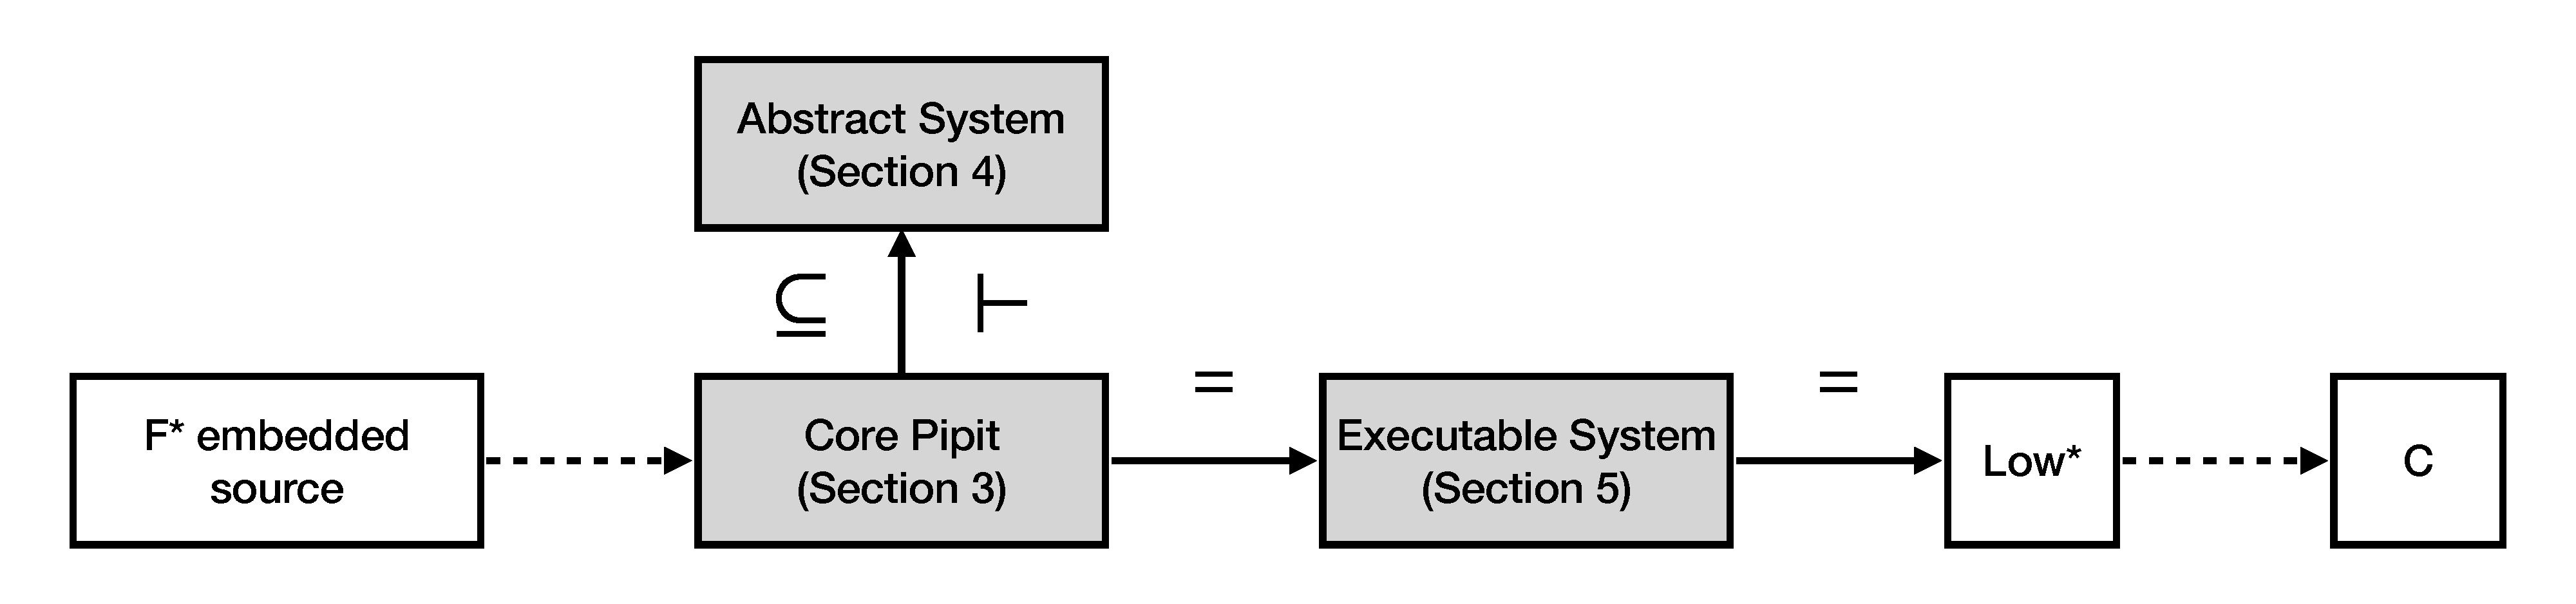
\includegraphics[width=\textwidth]{figures/core-structure-1920x450.pdf}
\caption{Architecture of Pipit. The gray boxes and solid arrows are defined in this paper. The white boxes and dashed arrows are trusted components. The labels next to the arrows denote verified properties of the translation: abstraction~($\subseteq$), entailment of proof obligations~($\vdash$), and equivalence~($=$).
% The refinement label ($\subseteq$) indicates a verified abstraction relation; the negated entailment ($\not\vdash$) indicates that the entailment relation --- that the proof obligations on the abstract transition system entail the original proof obligations --- is not yet verified; the equivalence ($=$) denotes a verified equivalence relation.
}
\label{f:core:structure}
\end{figure}
